%
% Report: Verilog-A Macromdel for Resistive Potentiometers
%
% Copyright (C) 2008 Mike Brinson <mbrin72043@yahoo.co.uk>
%
% Permission is granted to copy, distribute and/or modify this document
% under the terms of the GNU Free Documentation License, Version 1.1
% or any later version published by the Free Software Foundation.
%

% redefine subfigure caption
\renewcommand{\thesubfigure}{\thefigure(\alph{subfigure})}
\makeatletter
  \renewcommand{\@thesubfigure}{\thesubfigure:\space}
  \renewcommand{\p@subfigure}{}
\makeatother

% redefine subtable caption
\renewcommand{\thesubtable}{\thetable(\alph{subtable})}
\makeatletter
  \renewcommand{\@thesubtable}{\thesubtable:\space}
  \renewcommand{\p@subtable}{}
\makeatother

\tutsection{Introduction}

The resistive potentiometer is a common component in electronic
systems. Unfortunately, it is often very poorly modelled by circuit
simulators. A common approach is to simply treat the device as two
series resistances with values set by linear or logarithmic algebraic
equations.  This is fine as a rough and ready approach to modelling
the basic potentiometer function.  However, it fails to acknowledge
the fact that potentiometers are much more complex devices that
involve not only electrical characteristics but also mechanical
rotational features.  Furthermore, potentiometers are subject to a
number of errors such as taper conformity and linearity. This report
presents a more realistic model of a resistive potentiometer and shows
how Qucs can be used to develop practical models of this fundamental
component that give an order of magnitude improvement over the
commonly used two resistor models.  Finally, the notes show how a Qucs
subcircuit of the potentiometer can be coded as a compact Verilog-A
macromodel.


\tutsection{The two resistor potentiometer model}
The schematic for a two resister model of a linear resistive
potentiometer is shown in Fig.~\ref{fig:Pot1}. Sweep parameter
\textit{Position} is used to control the movement of the potentiometer
central output terminal. A range of zero to one covers the movement of
the output terminal from one end of the potentiometer to the
other. This model acts more like a sliding arm potentiometer rather
than the more common rotary type. Notice the use of non-integer values
1.00001 and 0.00001 to ensure that R1 or R2 do not become zero in
value when the mid-terminal is slid to either end of the
potentiometer.  Changing equations R1eqn and R2eqn allows different
laws to be specified that relate the values of resistors R1 and R2 to
the position of the mid-terminal.

\begin{figure} [here]
  \centering
  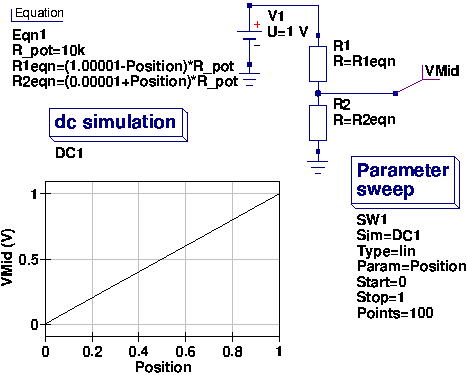
\includegraphics[width=0.5\linewidth]{Pot_Fig1}
  \caption{Basic two resistor model of a linear resistive potentiometer}
  \label{fig:Pot1}
\end{figure} 

\tutsection{Potentiometer types}
The basic types of resistive potentiometer are the rotary and slider
forms\footnote{R.G. Keen, The secret life of pots, 1999,
\url{http://www.geofex.com/Article_Folders/potsecrets/potscret.htm}
}. These are constructed from wire, cemet or conductive plastic
resistive strips attached to a suitable non-conducting holder with
fixed contacts at the ends and a moveable wiper contact. The moveable
contact either traverses in a rotary direction or in a straight
line. The resistive strip has either a constant width or is shaped
depending on the type of potentiometer, giving either constant
resistance or changing resistance per unit length along the length of
a potentiometer. Probably the most common of the non-linear types of
potentiometer is the logarithmic potentiometer. Figure~\ref{fig:Pot2}
illustrates how linear, logarithmic and inverse logarithmic device
laws vary as a function of wiper contact angle. Logarithmic
potentiometers are sometimes called audio potentiometers due to their
use as volume control devices in audio amplifiers. Potentiometers with
logarithmic resistive laws are necessary because the human ear
responds to the logarithm of loudness, making control of amplifier
output level smoother with a logarithmic potentiometer rather than the
simpler linear device. The shape of the potentiometer response law is
often called the potentiometer taper. Today linear potentiometers are
the most common type made by different manufacturers. One reason for
this is the cost of manufacturing a true logarithmic law device. In
many cases so called logarithmic potentiometers are in fact simpler
devices constructed from two different sections of resistive material
where the low angle part of the potentiometer track has a smaller
resistivity than the high angle section. Logarithmic potentiometers
are normally specified as 20\% or 10\% types, being defined as the
percentage of total potentiometer resistance between the bottom fixed
cantact and the wiper contact when the wiper is moved to the middle of
it's full range. Inverse logarithmic potentiometers have a similar
characteristic to the logarithmic potentiometer except that
potentiometer taper is reversed. This has the effect of causing large
changes in output at small wiper angles and the reverse at high
angles. Inverse logarithmic potentiometers have in recent years become
unusual items and are no longer widely manufactured.


\begin{figure} [here]
  \centering
  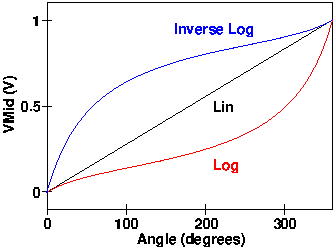
\includegraphics[width=0.4\linewidth]{Pot_Fig2}
  \caption{Resistive potentiometer characteristics: Vin = 1V DC}
  \label{fig:Pot2}
\end{figure} 


\tutsection{Modelling potentiometer taper laws}
Due to their lower cost, and availability, linear potentiometers are
often chosen as a starting point when designing a circuit that
requires a potentiometer with a specific taper law. The same applies
to modelling potentiometers with a known resistive taper. By adding a
fixed resistance, external to a potentiometer, a linear potentiometer
can be converted to one with a designer specified taper. Consider the
three resistor diagram shown in Fig.~\ref{fig:Pot3}.

\begin{figure} [here]
  \centering
  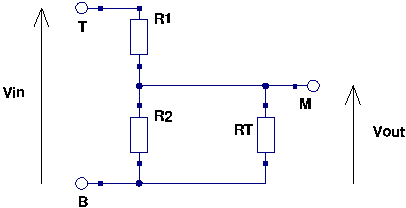
\includegraphics[width=0.6\linewidth]{Pot_Fig3}
  \caption{Basic two resister potentiometer with taper resister RT connect between the bottom fixed contact (B) and the wiper arm contact (M)}
  \label{fig:Pot3} 
\end{figure} 

The transfer function for the schematic illustrated in
Fig.~\ref{fig:Pot3} is given in equation \eqref{eq:pequ1}.

\begin{align}
\label{eq:pequ1}
\dfrac{Vout}{Vin}=\dfrac{\left( R_{2} \parallel R_{T} \right) }{R_{1}+\left( R_{2} \parallel R_{T} \right) }
                 =\dfrac{1}{1+\dfrac{R_{1}}{R_{T}}+\dfrac{R_{1}}{R_{T}}}
\end{align}  

Writing $Rpot=R_{1}+R_{2}$ and setting $a=R_{2}/Rpot$ and
$TaperCoeff=R_{T}/Rpot$ yields equation~\eqref{eq:pequ2}.

\begin{align}
\label{eq:pequ2}
\dfrac{Vout}{Vin}=\dfrac{1}{1+\dfrac{1-a}{a}+\dfrac{1-a}{TaperCoeff}}=\dfrac{a \cdot TaperCoeff}{a - a^{2} +TaperCoeff}
\end{align}  

Where $TaperCoeff$ is the potentiometer taper coefficient (a fixed
value greater than zero) and parameter $a$ is a measure of the wiper
arm position (being in the range 0 to 1). As the taper coefficient
approaches a large value (much greater than one) the potentiometer law
approaches that of a simple linear potentiometer, effectively this
implies that $R_{T}>>Rpot$.  For rotary potentiometers, parameter $a$
can also be expressed as $a=Angle/MaxAngle$. In the case of a single
turn potentiometer $0 <= Angle <= 360$ degrees and $MaxAngle = 360$
degrees.  Figure~\ref{fig:Pot4} illustrates the effect of different
$TaperCoeff$ values on the potentiometer response curves.  Logarithmic
potentiometer response is approximated when the $TaperCoeff$ is in the
range 0.2 to 0.25.

\begin{figure} [here]
  \centering
  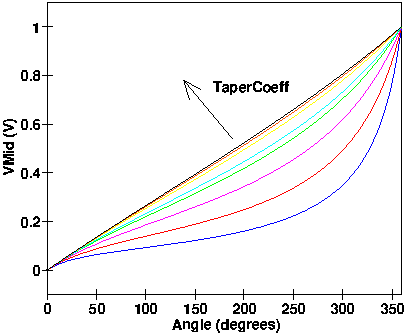
\includegraphics[width=0.6\linewidth]{Pot_Fig4}
  \caption{Potentiometer response curves for different $TaperCoeff$ values: curves blue to black; $TaperCoeff =$ 0.1, 0.2, 0.75, 1, 2, 3, 4, 5}
  \label{fig:Pot4}
\end{figure} 


\tutsection{Modelling inverse logarithmic potentiometers}
By placing the fixed taper resistance in parallel with resistor R1 the
potentiometer response changes to the inverse logarithmic form shown
in Fig.~\ref{fig:Pot2}. Consider the three resister model shown in
Fig.~\ref{fig:Pot5}.


\begin{figure} [here]
  \centering
  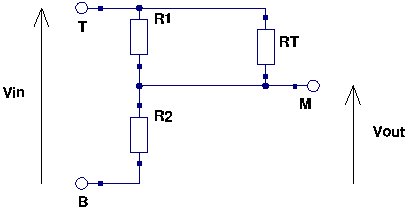
\includegraphics[width=0.6\linewidth]{Pot_Fig5}
  \caption{Basic two resister potentiometer with taper resister RT connect between the top fixed contact (T) and the wiper arm contact (M)}
  \label{fig:Pot5}
\end{figure} 
\medskip 

The transfer function for the schematic illustrated in
Fig.~\ref{fig:Pot5} is given in equation \eqref{eq:pequ3}.

\begin{align}
\label{eq:pequ3}
\dfrac{Vout}{Vin}=\dfrac{R_{2}} { \left( R_{1} \parallel R_{T} \right) + R_{2}}
                 =\dfrac{R_{2}} { \left( \dfrac{ R_{1} \cdot R_{T} } {R_{1} + R_{T} } \right)  + R_{2}  } 
                 =\dfrac{R_{1} \cdot R_{2} + R_{2} \cdot R_{T}}{R_{1} \cdot R_{2}+ R_{1} \cdot R_{T} + R_{2} \cdot R_{T}}
\end{align}  

Writing $Rpot=R_{1}+R_{2}$ and setting $a=R_{2}/Rpot$ and
$TaperCoeff=R_{T}/Rpot$ yields equation \eqref{eq:pequ4}.

\begin{align}
\label{eq:pequ4}
\dfrac{Vout}{Vin}=\dfrac{a - a^{2} + a\cdot TaperCoeff }{a - a^{2} + TaperCoeff}
\end{align}  

Figure~\ref{fig:Pot6} illustrates the effect of different $TaperCoeff$
values on the inverse potentiometer response curves.  Inverse
logarithmic potentiometer response is approximated when the
$TaperCoeff$ is in the range 0.2 to 0.25.


\begin{figure} [here] 
  \centering
  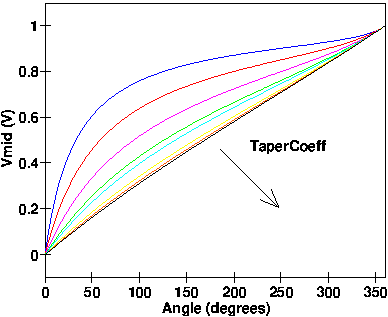
\includegraphics[width=0.6\linewidth]{Pot_Fig6}
  \caption{Inverse potentiometer response curves for different $TaperCoeff$ values: curves blue to black; $TaperCoeff =$ 0.1, 0.2, 0.75, 1, 2, 3, 4, 5}
  \label{fig:Pot6}
\end{figure} 



\tutsection{A Qucs subcircuit model of a resistive potentiometer}
The schematic for a resistive potentiometer modelled as a Qucs
subcircuit is shown in Fig.~\ref{fig:Pot7}. This model is based on the
background ideas and theory presented in the previous sections of this
report. The subcircuit schematic represents a practical resistive
potentiometer, with electrical and positional characteristics set by a
resistive taper coefficient, a conformity error parameter, a linearity
parameter, wiper arm contact resistance and resistance temperature
coefficient. The subcircuit models both single and multi-turn
potentiometers of type linear, logarithmic or inverse logarithmic and
indeed any other laws set by the value of parameter Taper\_Coeff.  The
following list outlines the function and units of the model
parameters.

\tutsubsection{Parameters}

\begin{longtable}{rllll}
Name & Symbol & Description & Unit & Default$^{*}$\\
\hline
\endhead
Rpot & $Rpot$ & Nominal device resistance & $\Omega$ & 1e4\\
Rotation & $Rotation$ & Shaft/wiper arm rotation & degrees & 120\\
Taper\_Coeff & $TaperCoeff$ & \parbox[t]{5.5cm}{Resistive law taper coefficient} & & 0\\
LEVEL & $LEVEL$ & Device type selector &  & 1$^+$\\
Temp& $Temp$ & Circuit temperature & Celsius  & 26.85\\
Max\_Rotation & $MaxRotation$ & \parbox[t]{5.5cm}{Maximum shaft/wiper rotation} & degrees  & 240$^{++}$\\
Conformity & $Conformity$ & Conformity error & \% & 0.2\\
Linearity & $Linearity$ & Linearity error & \% & 0.2\\
Tnom & $Tnom$ & \parbox[t]{5.5cm}{Parameter measurement temperature} & Celsius & 26.85\\
Contact\_Res & $ContactRes$ & \parbox[t]{5.5cm}{Wiper arm contact resistance resistance}  & $\Omega$ & 1\\
Temp\_Coeff & $TempCoeff$ & \parbox[t]{5.5cm}{Resistance temperature coefficient} & PPM/Celsius & 100$^{+++}$ \\
\end{longtable}

*  The default parameters are for typical 10k cemet linear potentiometer.  

+  Parameter LEVEL selects the potentiometer type: LEVEL=1; linear, LEVEL=2; logarithmic and LEVEL=3; inverse logarithmic.

++ For a single turn potentiometer 240 <= MaxRotation <= 360 degrees \footnote{The value of parameter MaxRotation is normally set by the position of an end stop at the end of the resistive track.}. For multi-turn potentiometers add 360 degrees per complete shaft rotation.

+++ Potentiometer temperature coefficients are normally quoted in parts per million (PPM) per degree Celsius by manufacturers. Typical values are: cemet $\pm$100 PPM/Celsius, wire $\pm$50 PPM/Celsius and conductive plastic $\pm$1000 PPM/Celsius. 

\bigskip

Potentiometer functional errors are introduced in the model
illustrated in Fig.~\ref{fig:Pot7} by adding conformity and linearity
factors to the basic taper coefficient via equation \eqref{eq:pequ5}.

\begin{align}
\label{eq:pequ5}
Tpcoeff=TaperCoeff+\dfrac{Conformity+Linearity\cdot \sin{\left( RadAngle  \right)}}{100}
\end{align}
Where $ RadAngle = Rotation \cdot \pi/180$ is the shaft rotation angle
in radians. Absolute conformity error is defined as the maximum
deviation of the taper function characteristic from an ideal
theoretical characteristic. Conformity error is normally specified in
percentage and can have plus or minus values. Absolute linearity has a
similar definition. However, it often shows sinusoidal
characteristics\footnote{See section 3.2: Novotechnik Potentiometer
Definitions,
\url{http://www.novotechnik.com/novotechnic_tech_ref.html}} due to
shaft rotation, particularly with multi-turn potentiometers. Contact
resistance has been introduced into the model to take account of any
resistance that exists from the wiper terminal to the contact on the
potentiometer resistive track. With sprung loaded contacts this
resistance should be small and can often be neglected. Effects of
temperature on the model performance are included via a simple linear
temperature coefficient which controls the change in device resistance
as temperature varies. A potentiometer test circuit and the response
of a multi-turn linear potentiometer with zero conformity and
linearity errors are given in Fig.~\ref{fig:Pot8}. Multi-turn
potentiometers are modelled by setting the shaft rotation parameter to
multiplies of 360 degrees plus slightly less angle for the final
rotation. Figure~\ref{fig:Pot9} illustrates a test circuit for
comparing the performace of log and inverse log single-turn
potentiometers. The response curves show both simulation results and
those obtained by fitting logarithmic curves to the simulated output
data. With the Taper\_Coeff parameter set to 0.2, remarkably good
agreement is observed when the simulation data is compared to the
ideal logarithmic performance. The test circuit and simulation curves
illustrated in Fig.~\ref{fig:Pot10} demonstrate the effects that
conformity and linearity parameters have on a multi-turn
potentiometer.  Normally both of these parameters are much less than
one percent, making their effects difficult to observe.  In
Fig.~\ref{fig:Pot10} they have both been set at ten percent, greatly
exaggerating their effect on potentiometer performance.

\begin{figure} [here] 
  \centering
  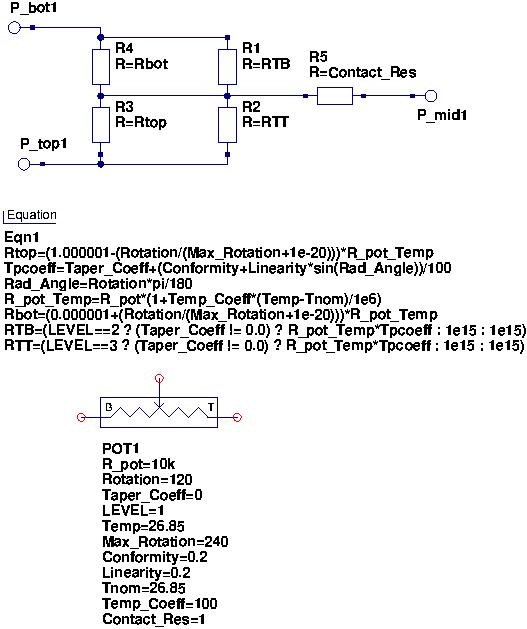
\includegraphics[width=0.7\linewidth]{Pot_Fig7}
  \caption{Qucs subcircuit of a resistive potentiometer: schematic, equations and symbol}
  \label{fig:Pot7}
\end{figure} 

\begin{figure} [here] 
  \centering
  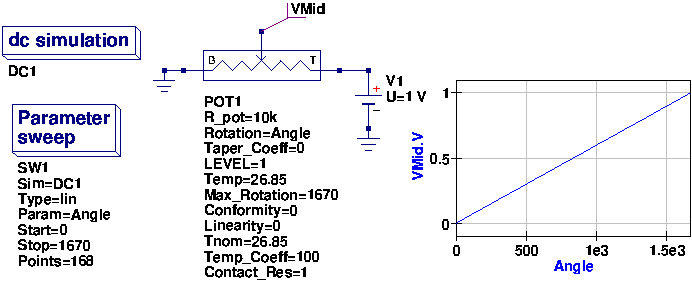
\includegraphics[width=0.9\linewidth]{Pot_Fig8}
  \caption{Multi-turn linear potentiometer test circuit and performance curve}
  \label{fig:Pot8}
\end{figure} 


\begin{figure} [here]  
  \centering
  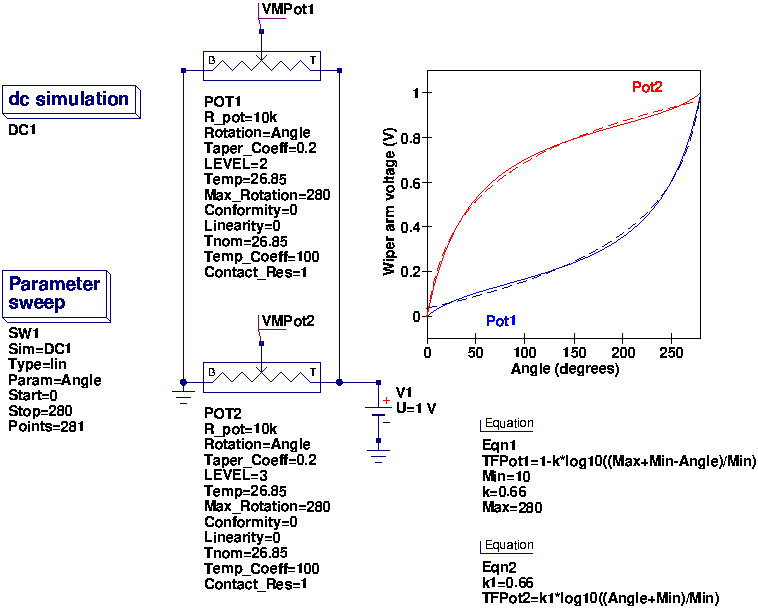
\includegraphics[width=0.9\linewidth]{Pot_Fig9}
  \caption{Single-turn log and inverse log potentiometer test circuit and performance curves: (1) simulated data  solid curves, (2) fitted data dotted curves}
  \label{fig:Pot9}
\end{figure} 


\begin{figure} [here] 
  \centering
  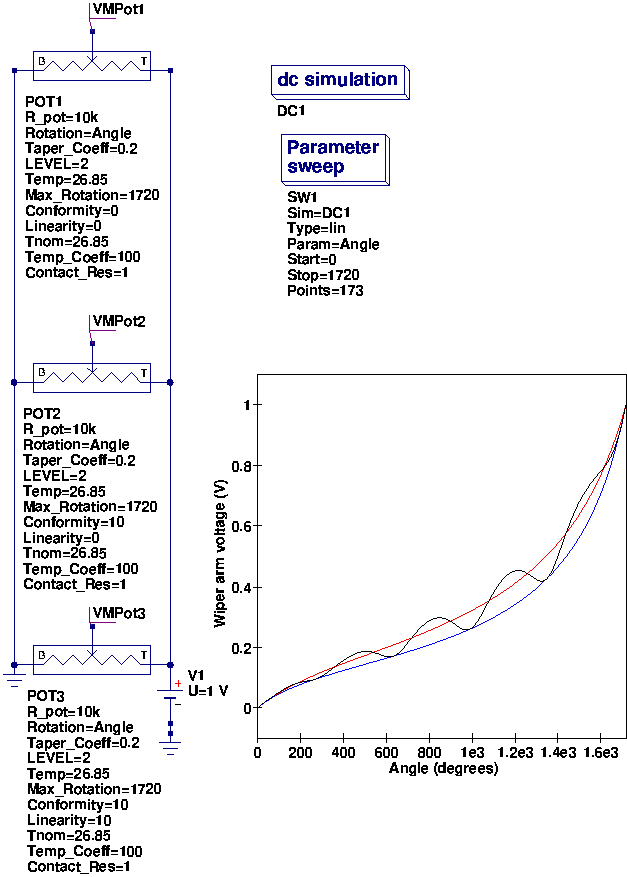
\includegraphics[width=0.9\linewidth]{Pot_Fig10}
  \caption{Multi-turn log potentiometer test circuit and response curves, illustrating conformity and linearity errors: both conformity and linearity parameters are set at ten percent to clearly indicate their effects; blue curve Pot1, red curve Pot2 and black curve Pot3}
  \label{fig:Pot10}
\end{figure} 



\tutsection{A Verilog-A resistive potentiometer model}
One of the advantages of using Qucs subcircuits, and indeed EDD
models, is that they allow fast interactive prototyping of new models.
Once a new model is tested and functioning satisfactorily it can often
be easily translated into Verilog-A code for compiling into C++ code,
using the ADMS compiler, and finally compiled and linked with the main
Qucs software. When prototyping new models it is advisable to use,
whenever possible, circuit elements/structures that can be easily
transposed to Verilog-A statements.  The Verilog-A code listed in the
next section is based directly on the Qucs subcircuit model of the
potentiometer. In general there is a one-to-one correspondence between
the different sections of the subcircuit model and the Verilog-A code.
However, for completeness the Verilog-A code also includes white noise
statements to account for resistor noise\footnote{The resistors
comprising the potentiometer subcircuit have thermal noise built-in as
a standard component feature.}.  Overall the subcircuit model and the
Verilog-A code give the same performance except that the Verilog-A
code appears to simulate much faster. This is not surprising
considering it comprises compiled and linked machine code rather than
being a netlist which is interpreted during circuit simulation.

\tutsection{Verilog-A model code}

\begin{lstlisting}[
 language=Verilog, 
 xleftmargin=12pt,
 basicstyle=\scriptsize]
//   Qucs resistive potentiometer model:
//   This model can be used to construct working linear, logarithmic and inverse logarithmic
//   potentiometers, or other devices with designer specified resistive taper functions.
//   All required parameters can be extracted directly from
//   manufacturers data sheets.
//
//   The structure and theoretical background to the potentiometer
//   Verilog-a model are presented in the Qucs potentiometer report.
//
//   This is free software; you can redistribute it and/or modify
//   it under the terms of the GNU General Public License as published by
//   the Free Software Foundation; either version 2, or (at your option)
//   any later version.
// 
//   Copyright (C), Mike Brinson, mbrin72043@yahoo.co.uk, February 2008.
//
`include "disciplines.vams"
`include "constants.vams"
// 
 module potentiometer (B, M, T);
 inout B, M, T;
//
 electrical B, M, T;
//
// Internal nodes
//
 electrical n1;
//
 `define attr(txt) (*txt*)
//
 parameter real R_pot = 1e4 from [1e-6 : inf]
  `attr(info="nominal device resistance" unit = "Ohm");
 parameter real Rotation = 120 from [0 : inf]
  `attr(info="shaft/wiper arm rotation" unit = "degrees");
 parameter real Taper_Coeff = 0 from [0 : inf]
  `attr(info="resistive law taper coefficient" );
 parameter integer LEVEL = 1 from [1 : 3]
  `attr(info="device type selector" );
 parameter real Max_Rotation = 240.0 from [0 : inf]
  `attr(info="maximum shaft/wiper rotation" unit = "degrees");
 parameter real Conformity = 0.2 from [-inf : inf]
  `attr(info="conformity error" unit = "%");
 parameter real Linearity = 0.2 from [-inf : inf]
  `attr(info="linearity error" unit = "%");
 parameter real Contact_Res = 1 from [1e-6 : inf]
  `attr(info="wiper arm contact resistance" unit = "Ohm");
 parameter real Temp_Coeff = 100 from [0 : inf]
  `attr(info="resistance temperature coefficient" unit = "PPM/Celsius");
 parameter real Tnom = 26.85 from [-273 : inf]
  `attr(info="parameter measurement temperature" unit = "Celsius");
//
real Rad_Angle, R_pot_Temp, Rtop, Rbot, Tpcoeff, Rcontact;
real RTB, RTT, error_term;
real fourkt;
//
analog begin
//
// Model equations
//
Rcontact=Contact_Res+1e-6;
Rad_Angle=Rotation*`M_PI/180;
R_pot_Temp=(R_pot+1e-6)*(1+Temp_Coeff*($temperature-Tnom)/1e6);
Tpcoeff=Taper_Coeff+(Conformity+Linearity*sin(Rad_Angle))/100;
error_term=(1+(Conformity+Linearity*sin(Rad_Angle))/100);
//
case (LEVEL)
   2: begin
	RTB=R_pot_Temp*Tpcoeff;
	RTT=1e15;
        Rtop=(1.000001-(Rotation/(Max_Rotation+1e-20)))*R_pot_Temp;
        Rbot=(0.000001+(Rotation/(Max_Rotation+1e-20)))*R_pot_Temp;
      end
   3: begin
	RTB=1e15;
	RTT=R_pot_Temp*Tpcoeff;
        Rtop=(1.000001-(Rotation/(Max_Rotation+1e-20)))*R_pot_Temp;
        Rbot=(0.000001+(Rotation/(Max_Rotation+1e-20)))*R_pot_Temp;

      end
  default:begin
        RTB=1e15;
        RTT=1e15;
        Rtop=(1.000001-(Rotation/(Max_Rotation+1e-20)))*R_pot_Temp*error_term;
        Rbot=(0.000001+(Rotation/(Max_Rotation+1e-20)))*R_pot_Temp*error_term;

      end
endcase
//
if (Taper_Coeff == 0.0) 
 begin 
   RTB=1e15;
   RTT=1e15;
   Rtop=(1.000001-(Rotation/(Max_Rotation+1e-20)))*R_pot_Temp*error_term;
   Rbot=(0.000001+(Rotation/(Max_Rotation+1e-20)))*R_pot_Temp*error_term;
 end
//
// Macromodel
//
I(T, n1) <+ V(T, n1)/Rtop;
I(T, n1) <+ V(T, n1)/RTT;
I(B, n1) <+ V(B, n1)/Rbot;
I(B, n1) <+ V(B, n1)/RTB;
I(M, n1) <+ V(M, n1)/Rcontact;
//
// Noise contributions
//
fourkt=4.0*`P_K*$temperature;
I(T, n1) <+ white_noise(fourkt/Rtop, "thermal");
I(T, n1) <+ white_noise(fourkt/RTT, "thermal");
I(B, n1) <+ white_noise(fourkt/Rbot, "thermal");
I(B, n1) <+ white_noise(fourkt/RTB, "thermal");
I(M, n1) <+ white_noise(fourkt/Rcontact, "thermal");

//
end
endmodule
\end{lstlisting}

The ADMS syntax is a subset of Verilog-A.  Allowed language structures
are outlined in a SYNTAX-SUPPORTED file which can be downloaded from
\url{http://mot-adms.sourceforge.net}. Recent news concerning the ADMS
Verilog-A compiler can also be found on the ADMS Website Wiki.

\tutsection{End note}
Resistive potentiometers are fundamental components in electronic
system design. They deserve due attention when forming part of a
circuit simulation package.  This report introduces a number of basic
properties of potentiometric devices and outlines how they can be
accurately and efficiently simulated by Qucs. While writing this
report I have tried to demonstrate how practical resistive
potentiometer models can be constructed from a set of basic concepts.
Qucs subcircuits and component defining equations form the fundamental
tools for modelling a potentiometer. Both encourage interactive model
development and the subsequent conversion of their properties into
Verilog-A code.  My thanks to Stefan Jahn for all his help and
encouragement during the period I have been working on the
potentiometer model and writing this report.



